\documentclass{article}

\usepackage{polski}
\usepackage[utf8]{inputenc}
\usepackage{graphicx}
\usepackage{amsthm}


\title{\centering \Large Analiza Numerczna - zadanie 2.14 \\
\large Wyprowadzanie i implementacja hiperoblicznej funkcji sklejanej}

\author{\Large Prowadzący: Paweł Woźny\thanks{\textit{E-mail}: \texttt{Pawel.Wozny@ii.uni.wroc.pl}}%
	    \and \Large autor: Dawid Więcław}

\addtolength{\textwidth}{4cm}
\addtolength{\hoffset}{-2cm}
\addtolength{\textheight}{4cm}
\addtolength{\voffset}{-2cm}

\begin{document}
\maketitle
\thispagestyle{empty}
\setcounter{page}{1}
\section{Wstęp}
\subsection{Co to jest hiperboliczna funkcja sklejana?}
\large
\hspace{3mm} Hiperboliczna funkcja sklejana jest to funkcja określona na przedziałach (pomiędzy węzłami), gdzie interpoluje ona zadaną wcześniej funkcję, której wartości w punktach pośrednich są nieznane bądź trudne do wyliczenia. Hiperboliczną funkcję sklejaną interpolującą odróżnia, od klasycznych funkcji interpolujących, parametr $\tau$, który pozwala na wygładzenie jej wykresu odpowiednio dostosowując ją do potrzeb osoby interpolującej.

\subsection{Zastosowanie interpolującej, hiperbolicznej funkcji sklejanej}
\hspace{3mm} Funkcje omawiane w tym sprawozdaniu mają zastosowanie w przybliżaniu funkcji (jak każda interpolująca funkcja), jednakże poprzez możliwość zmiany "napięcia", czyli wygładzenia jej wykresu można odnaleźć zastosowanie tej funkcji w grafice komputerowej.
Kolejnym przykładem zastosowania tych funkcji są rozważania na temat silników elektrycznych, a mianowicie jego parametrów - napięcia wzbudzenia w zależności od napięcia twornika i momentu obrotowego silnika elektrycznego obcowzbudnego. Właściwie w przypadku każdych dyskretnych danych, wiedząc jak powinna kształtować się zależność (jak bardzo funkcja powinna być wygładzona) użycie interpolującej hiperbolicznej funkcji sklejanej może mieć zastosowanie w celu określenia tej zależności.
\subsection{Wzór}
$S_{\tau}=\frac{M_{k}sinh(\tau x_{k+1}-\tau x)}{sinh(\tau h_{k})} + \frac{M_{k+1}sinh(\tau x - \tau x_{k})}{sinh(\tau h_{k})} + \frac{(f(x_{k})-M_{k})(x_{k+1}-x)}{h_{k}} + \frac{f(x_{k+1}-M_{k+1})(x-x_{k})}{h_{k}}$
\newline
\newline
Gdzie:
\begin{enumerate}
\item $h_{k}=x_{k+1}-x_{k}$
\item $M_{k}=\frac{S_{\tau}''(x_{i})}{r^{2}}$
\end{enumerate}
\subsection{Na czym polega eksperyment?}
Eksperyment polega na zaimplementowaniu algorytmu wyznaczania hiperbolicznej sklejanej funkcji interpolującej i przetestowanie jej do przybliżania różnych funkcji a także wyznaczenie kilku rysunków dla danych w postaci dyskretnej dla różnych $\tau$.
\newpage
\section{Uzyskiwanie hiperbolicznej funkcji skelejanej}
\subsection{Warunki które musi spełniać hiperboliczna funkcja interpolacyjna}
\begin{enumerate}
\item $S_{\tau} \in C^{2}[a.b]$
\item $S_{\tau}(x_{k}) = f(x_{k})$
\item dla $x \in (x_{k}, x_{k+1})$ $S_{\tau}^{(4)}(x)-\tau^{2}S_{\tau}''(x)=0$
\end{enumerate}
\subsection{Wyprowadzenie}
\subsubsection{Wzór na funkcję}
Rozpocznijmy od równiania różniczkowego: 
$S_{\tau}^{(4)}(x)=\tau^{2}S_{\tau}''(x)$, podstawiając $S_{\tau}(x) = e^{\lambda x}$ 
otrzymujemy wynik równania różniczkowego w postaci ogólnej: $S_{\tau}(x)=ae^{\tau x}+be^{-\tau x}+cx+d$. Wniskując z postaci ogólnej otrzymuje się: $S_{\tau}''(x)=a \tau^2e^{\tau x} + b \tau^2e^{-\tau x}=\tau^2(ae^{\tau x} + be^{-\tau x})$, dzięki możliwości skorzystania z wartości pomocniczej $M_{k}=\frac{S_{\tau}''(x_k)}{\tau^2}$ można przedstawić drugą pochodną funkcji $S_{\tau}$ na przedziale [$x_k$,$x_{k+1}$] w postaci: 
\newline
$S_{\tau}''(x)=M_{k} \tau^2sinh^{-1}(\tau h_k)sinh(\tau(x_{k+1}-x))+M_{k+1} \tau^2sinh^{-1}(\tau h_k)sinh(\tau(x-x_k))$ 
\newline
Po podwojnym scałkowaniu tej funkcji otzymujemy postać: 
\newline
$S_{\tau}(x)=M_{k} sinh^{-1}(\tau h_k)sinh(\tau(x_{k+1}-x))+M_{k+1} sinh^{-1}(\tau h_k)sinh(\tau(x-x_k))+Ax+B$
Jednakże znając wartość funkcji $S_{\tau}(x)$ w puntkach $x_k$ i $x_{k+1}$, z układu równań wywnioskować ostateczną postać funkcji:
\newline
$S_{\tau}=\frac{M_{k}sinh(\tau x_{k+1}-\tau x)}{sinh(\tau h_{k})} + \frac{M_{k+1}sinh(\tau x - \tau x_{k})}{sinh(\tau h_{k})} + \frac{(f(x_{k})-M_{k})(x_{k+1}-x)}{h_{k}} + \frac{(f(x_{k+1})-M_{k+1})(x-x_{k})}{h_{k}}$
\subsubsection{Jak wyliczyć $M_k$?}
Ciagłość funkcji $S_{\tau}(x)$ jest zagwarantowana co można łatwo uduwodnić z jej wzoru obliczając $S_{\tau}(x_{k}+0)$ i $S_{\tau}(x_{k}-0)$, ciągłość $S''_{\tau}(x)$ można udowodnić w ten sam sposób. Pozostaje jedynie pozostaje jedynie wyznaczyć $M_{k}$ tak, aby zachować ciągłość $S'_{\tau}(x)$.
Rozpatrując pierwszą pochodną rozważanej funkcji na przedziałach $[x_{k}, x_{k+1}]$ i $[x_{k-1}, x_{k}]$ otrzymuje się wzory:
\begin{enumerate}
\item $S_{\tau}(x)=-\tau M_{k} \frac{cosh(\tau x_{k+1} - \tau x)}{sinh(\tau h_{k})} + \tau M_{k+1} \frac{cosh(\tau x - \tau x_{k})}{sinh(\tau h_{k})} - \frac{f(x_{k})-M_{k}}{h_{k}} + \frac{f(x_{k+1}) - M_{k+1}}{h_{k}}$
\item $S_{\tau}(x)=-\tau M_{k-1} \frac{cosh(\tau x_{k} - \tau x)}{sinh(\tau h_{k-1})} + \tau M_{k} \frac{cosh(\tau x - \tau x_{k-1})}{sinh(\tau h_{k-1})} - \frac{f(x_{k-1})-M_{k-1}}{h_{k-1}} + \frac{f(x_{k}) - M_{k}}{h_{k-1}}$
\end{enumerate}
Odejmując je do siebie stronami otrzymuje się równanie:
\newline
$\alpha_{k-1}M_{k-1} + (\beta_{k-1} + \beta_{k}) M_{k} + \alpha_{k}M_{k+1} = \gamma_{k}- \gamma_{k-1}$
\newline
Gdzie z kolei:
\begin{enumerate}
\item $h_{k} = x_{k+1} - x_{k}$
\item $\alpha_{k} = \frac{1}{h_{k}} - \frac{\tau}{sinh(\tau h_{k})}$
\item $\beta_{k} = \frac{\tau cosh(\tau h_{k})}{sinh(\tau h_{k})} - \frac{1}{h_{k}}$
\item $\gamma_{k} = \frac{f(x_{k+1} - f(x_{k})}{x_{k+1}-x_{k}}$
\end{enumerate}
Rozważając to równanie dla $1 \leq k \leq n-1$ oraz zakładając $M_{0}=M{n}=0$ otrzymuje się układ równań pozwalający uzyskać wszystkie wartości $M_{k}$.

\newpage
\section{Implementacja}
\subsection{struktury pomocnicze}
W programie zostały napisane pomocnicze funkcje i struktury danych:
\begin{enumerate}
\item $X[i]$ -- tablica zwracająca i-ty argument $(x_{i})$
\item $alpha(i)$, $beta(i)$, $gamma(i)$ zwracające odpowiednio $\alpha_{i}$, $\beta_{i}$, $\gamma_{i}$. 
\item $h(k)$ zwracająca wartość wyrażenia $x_{k+1}-x_{k}$
\item $sinh(x)$ i $cosh(x)$ zwracające odpowiednio wartości tych funkcji dla argumentu x
\item $y(i)$ zwracająca wartość $\gamma_{i}-\gamma_{i-1}$
\item $findXi(x)$ zwracająca $k$, takie że $x \in [x_{k}, x_{k+1}]$
\end{enumerate}
\subsection{Główna część algorytmu wyznaczającego parametry hiperbolicznej funkcji sklejanej}
Parametry $M_{k}$ są trzymane w tablicy $M[]$ i wyliczane są w następujących etapach
\begin{enumerate}
\item Uzupełnienie tablicy $Y[]$ przez przypisanie $Y[i]=y(i)$, funkcja $y(i)$ została zaś już zdefiniowana, a przypisanie odbywa się w metodzie $fillY()$.
\item Uzupełnienie tablicy pomocniczej $T[]$ wartościami odpowiednio $\beta_{0} + \beta_{1}$, $\alpha_{1}$, $\beta_{1} + \beta_{2}$, ... , $\alpha_{n-2}$, $\beta_{n-1} + \beta_{n}$. Wypełnienie tablicy $T$ odbywa się w funkcji $fillT()$
\item Wykonanie zmodyfikowanej eleminacji Gaussa dla układu równań poprzez modyfikacje elementów tablic $Y$ i $T$ w celu ustalenia wartośći $M_{n-1}$
\item Ponowne wywołanie funkcji $fillY$ i $fillT$ w celu uzyskania wartości $M_{k}$ dla $k = n-2, n-3, ... , 2, 1$. 
\end{enumerate} 
\subsection{Implementacja hiperbolicznej funckcji sklejanej interpolacyjnej}
Funkcja $Sr(x)$ jest reprezentacją $S_{\tau}(x)$, a jej działanie polega na wywołaniu metody $findXi(x)$ w celu znalezienia rozpatrywanego przedziału, następne obliczane są wartości $a = \frac{M_{k}sinh(\tau x_{k+1}-\tau x)}{sinh(\tau h_{k})} $, $b = \frac{M_{k+1}sinh(\tau x - \tau x_{k})}{sinh(\tau h_{k})}$, $c = \frac{(f(x_{k})-M_{k})(x_{k+1}-x)}{h_{k}}$ oraz $d = \frac{(f(x_{k+1})-M_{k+1})(x-x_{k})}{h_{k}}$ reprezentujące składniki sumy zwracanej przez funkcję $S_{\tau}(x)$ (zostało to rozbite na aż 4 składniki aby funkcja była bardziej czytelna i łatwiejsze było znalezienie błędów). Następnie zwracana jest suma $a+b+c+d$.

\newpage

\section{Testy}
\subsection{Dla zbioru dyskretnego -- próba odtworzenia rysunku 6.5 a i 6.5 b z książki D. Kincaid, W. Cheney, Analiza numeryczna, WNT, 2005}
W tym przypadku interpolacja będzie przebiegała na funkcji która zwraca tylko wartości w punktach $x_{k}$, a w pozostałych nie jest ona zdefiniowana. W ten sposób dzięki hiperbolicznym funkcjom sklejanym interpolacyjnym można uzyskiwać różne rysunki (na przykład samochód).
\begin{figure}[ht]
  \begin{center}
  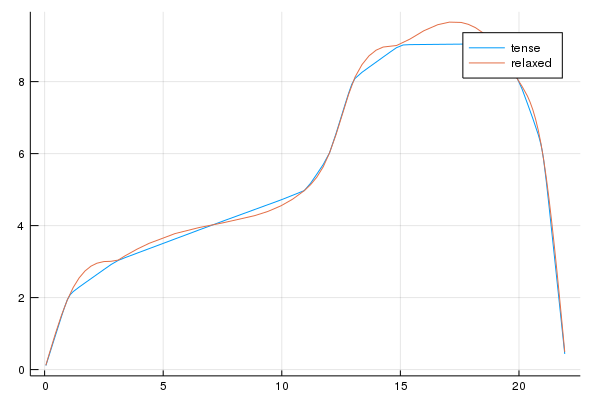
\includegraphics[width=15cm]{samochodzik}
  \end{center}
  \caption{Niebieski wykres został wykonany dla $\tau = 10$, pomarańczowy zaś dla $\tau = 0.1$. Dzięki temu udało ukazać się różnice wynikające ze zmiany stopnia napięcia wykresu}
  \label{fig:rysunek}
\end{figure}
\newpage
\subsection{Prostszy test dla zbióru dyskretnego}
Jest to kolejny przypadek próby narysowania wykresu funkcji zdefiniowanej tylko w poszczególnych punktach, tym razem przykład jest uproszczony aby lepiej można było dostrzec różnice między poszczególnymi stopniami napięcia.
\begin{figure}[ht]
  \begin{center}
  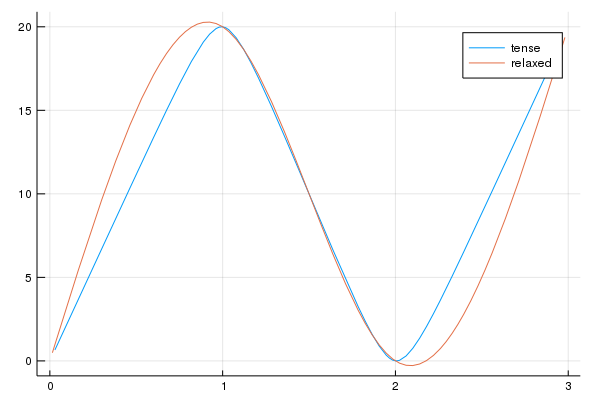
\includegraphics[width=15cm]{zbiorDyskretny}
  \end{center}
  \caption{Niebieski wykres został wykonany dla $\tau = 10$, pomarańczowy zaś dla $\tau = 0.1$.}
  \label{fig:rysunek}
\end{figure}
\newpage
\subsection{Pierwsza próba interpolacji funkcji}
Hiperboliczne funkcje sklejane mają również zastosowanie w klasycznej interpolacji funkcji, dzięki współczynnikowi $\tau$ można uzyskać nawet lepsze przybliżenia dla wyników jakiegoś eksperymentu niż sama funkcja matematyczna, gdyż przy pomocy tension spline można uzyskać niemal dowolne przybliżenie funkcji oryginalnej, a jednocześnie pozwala ją dość swobodnie modyfikować.
\begin{figure}[ht]
  \begin{center}
  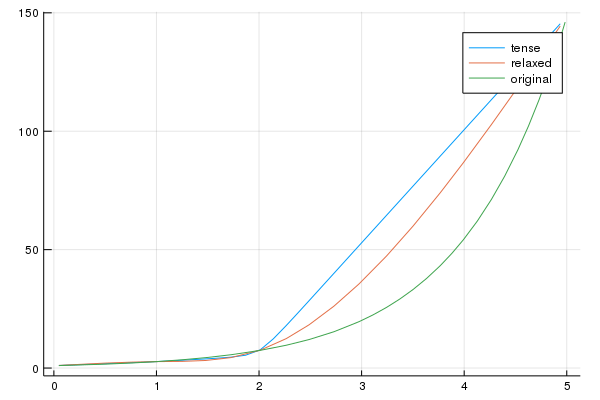
\includegraphics[width=15cm]{edox}
  \end{center}
  \caption{Niebieski wykres został wykonany dla $\tau = 10$, pomarańczowy dla $\tau = 0.1$, a na zielono została narysowana oryginalna funkcja.}
  \label{fig:rysunek}
\end{figure}
\newpage
\subsection{Druga próba interpolacji funkcji}
Tym razem jako funkcję interpolowaną zastosowano $f(x) = sin(x)$.
\begin{figure}[ht]
  \begin{center}
  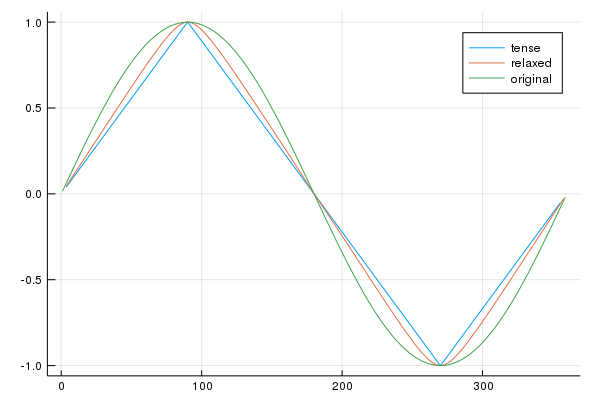
\includegraphics[width=15cm]{sin}
  \end{center}
  \caption{Niebieski wykres został wykonany dla $\tau = 10$, pomarańczowy dla $\tau = 0.1$, a na zielono zostałą naryoswana oryginalna funkcja.}
  \label{fig:rysunek}
\end{figure}
\newpage
\section{Co się dzieje po zwiększeniu liczby punktów?}
\begin{figure}[ht]
  \begin{center}
  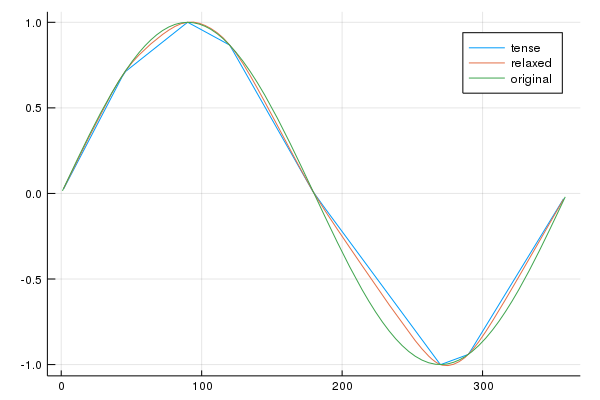
\includegraphics[width=11cm]{sin1}
  \end{center}
  \caption{Interpolwoanie funkcji sin(x) w większej liczbie punktów}
  \label{fig:rysunek}
\end{figure}

\begin{figure}[h]
  \begin{center}
  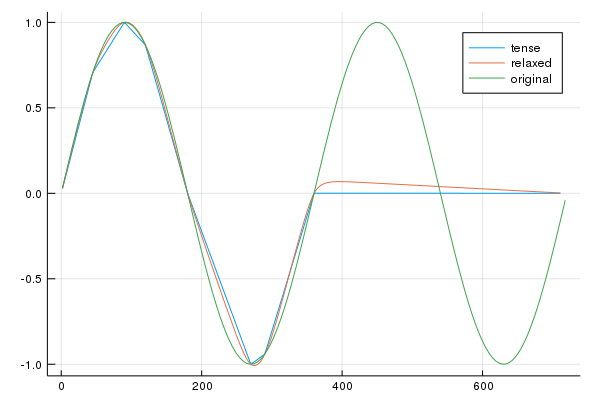
\includegraphics[width=11cm]{sin2}
  \end{center}
  \caption{Poszerzenie rozpatrywanego przedziału}
  \label{fig:rysunek}
\end{figure}
Zwiększenie liczby punktów w przypadku interpolacyjnych funkcji sklejanych zawsze poprawia przybliżenie danej funkcji z tego względu, że przybliżenia mogą być rozpatrywane na mniejszych przedziałach, a funkcja interpolacyjna osiąga wartości takie same jak wartości funkcji w węzłach. Dzięki zmniejszeniu przedziałów na których funkcja jest interpolowana, a dla każdego przedziału funkcję sklejaną dostosowuje się osobno jedynie zachowując konieczne założenia, interpolacja z każdym zwiększeniem liczby punktów jest dokładniejsza. To powoduje ,że odpowiednio zwiększając liczbę punktów można uzyskać dowolne przybliżenie interpolowanej funkcji (ograniczeniem jest jedynie pamięć komputera). Dodatkowym przyspieszeniem interpolacji jest modyfikacja $\tau$ co sprawia ,że wykres wygląda na jeszce bardziej zbliżony do funkcji bazowej i "naturalny", czyli bez ostrych krawędzi i wygładzony.

\section{Podsumowanie}
Interpolacyjne funkcje sklejane hiperboliczne pozwalają na przybliżanie dowolnej funkcji zadanej w dowolny sposób (wystarczy znać jej wartości w punktach w których chcemy ją interpolować), a także dzięki czynnikowi $\tau$ można modyfikować jej kształt bez zmiany węzłów interpolacji. Te zmiany estetyczne pozwalają na lepsze dostosowanie zachowania funkcji do osiąganych wyników eksperymentu lub mogą mieć zastosowanie w grafice. Jednakże nie jest to sposób lepszy pod każdym wzgledem od klasycznej interpolacji, gdyż zapamiętanie wszystkich wartości $M_{k}$ wymaga więcej pamięci niż zastosowanie wielomianu interpolacyjnego, a także znalezienie wartości funkcji sklejanej wymaga więcej czasu, ponieważ należy najpierw znaleźć przedział $[x_{k}, x_{k+1}]$, do którego należy dany argument.
\end{document}
